\section{Instrumental de trabajo}
Para el desarrollo, integración y validación del prototipo se utilizará el siguiente instrumental y equipamiento de laboratorio:

\begin{itemize}
	\item \textbf{PC de desarrollo:} estación de trabajo con entorno de compilación, programación y depuración del firmware, control de versiones y documentación.
	\item \textbf{Fuente de alimentación de laboratorio:} fuente regulable con limitación de corriente para pruebas seguras del prototipo y de sus rieles de alimentación.
	\item \textbf{Osciloscopio digital:} para verificación de formas de onda, medición de amplitud, offset, tiempos de transición y jitter. Se emplearán sondas pasivas y, cuando corresponda, terminación de 50\,$\Omega$.
	\item \textbf{Multímetro digital TRMS:} para mediciones de tensión y corriente en continua y alterna, y verificación de rieles de alimentación.
	\item \textbf{Analizador de espectro / FFT de osciloscopio:} para caracterización espectral (armónicos, espurios) y estimación de métricas como THD y SFDR, si se dispone.
	\item \textbf{Cargas y terminaciones:} resistencias de potencia, terminaciones coaxiales de 50\,$\Omega$, y condición High-Z (1\,M$\Omega$) para ensayos comparativos.
	\item \textbf{Cables y conectividad:} cables coaxiales BNC cortos, adaptadores, conectores, pinzas y puntas de prueba para minimizar errores de medición.
	\item \textbf{Herramientas de montaje y retrabajo:} estación de soldado, estación de aire caliente, flux, estaño, lupa/microscopio, y consumibles para ensamblado SMD.
	\item \textbf{Instrumental para verificación de componentes}.
\end{itemize}

En particular se va a utilizar el osciloscopio \textbf{OWON VDS1022I}. Puede verse una imagen ilustrativa a continuación.

\begin{figure}[H]
	\centering
	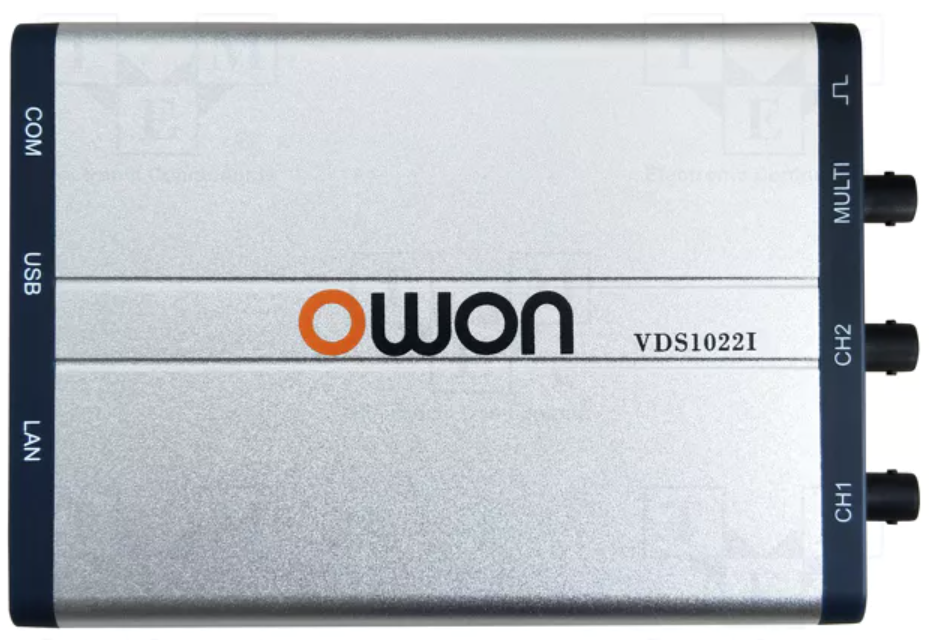
\includegraphics[width=0.7\linewidth]{Comparacion/img/owon_vds1022i}
	\caption{Osciloscopio OWON VDS1022I.}
	\label{fig:owonvds1022i}
\end{figure}

\paragraph{OWON VDS1022I (osciloscopio USB aislado para PC):}
Es un osciloscopio digital basado en PC, de \textbf{2 canales} con \textbf{aislación por USB}, orientado a mediciones generales y portabilidad.

\begin{itemize}
	\item \textbf{Canales:} 2 + 1 (entrada externa / multifunción). 
	\item \textbf{Ancho de banda analógico:} 25\,MHz.
	\item \textbf{Tasa de muestreo en tiempo real:} 100\,MSa/s.
	\item \textbf{Resolución vertical (ADC):} 8\,bits (2 canales simultáneos).
	\item \textbf{Memoria / record length:} 5\,kpts.
	\item \textbf{Base de tiempos:} 5\,ns/div a 100\,s/div (pasos 1--2--5).
	\item \textbf{Sensibilidad vertical:} 5\,mV/div a 5\,V/div.
	\item \textbf{Impedancia de entrada:} 1\,M$\Omega$ en paralelo con $\sim$10\,pF.
	\item \textbf{Acoplamiento de entrada:} DC, AC y GND.
	\item \textbf{Tensión máxima de entrada:} hasta 400\,V (pico a pico), según condición de medición/probador.
	\item \textbf{Modos de adquisición:} sample, peak detect y average.
	\item \textbf{Disparos (trigger):} edge, pulse, video, slope y alternate; modos auto/normal/single.
	\item \textbf{Funciones matemáticas:} suma, resta, multiplicación, división, inversión y FFT; vistas FFT y X--Y.
	\item \textbf{Interfaz:} USB 2.0 con \textbf{aislación} (menor interferencia y protección de la PC).
	\item \textbf{Alimentación:} por bus USB (no requiere fuente externa).
\end{itemize}